\documentclass[12pt]{article}

\usepackage{graphicx}
\usepackage{hyperref}
\usepackage{listings}

\setlength{\textheight}{8.5in}
\setlength{\headheight}{.25in}
\setlength{\headsep}{.25in}
\setlength{\topmargin}{0in}
\setlength{\textwidth}{6.5in}
\setlength{\oddsidemargin}{0in}
\setlength{\evensidemargin}{0in}

\title{PartyUp Internals}
\author{David Gilhooley, Lance Goodridge, Blake Lawson, and Graham Turk}
\begin{document}

\pagestyle{plain}

\maketitle

%%---------------------------------------------------------------------------------------------------
%% Introduction
%%---------------------------------------------------------------------------------------------------

\section{Overview}

PartyUp is an iOS app written in Swift.
The app's back end is hosted on an Amazon Web Services (AWS)
EC2 instance running Ubuntu.
The back end is built using the Django web framework and uses
a MySQL database.
PartyUp uses Git for version control and the code for the project is 
hosted on \href{https://github.com/}{GitHub}.
The iOS code and back end code can be found at 
\url{https://github.com/BDGL-Hacks/iOS-333} and
\url{https://github.com/BDGL-Hacks/backend-333} respectively.

The front end iOS app interacts with the back end API through HTTP requests.
The iOS client sends a POST request to the Django application on the AWS instance
that indicates which API function to call, and the server returns a JSON object that 
includes the information requested by the client.
All of the functions in the PartyUp API are documented on GitHub
in the project wiki (\url{https://github.com/BDGL-Hacks/backend-333/wiki}).

%%---------------------------------------------------------------------------------------------------
%% Front End
%%---------------------------------------------------------------------------------------------------

\section{Implementation: Front End}

\subsection{Code Structure}
The project's iOS code is written in the Swift programming language in the Xcode development environment.
You can build and run the project using one of the simulators in Xcode or
by plugging in a registered Apple device.
The code design follows the traditional Model-View-Controller (MVC) paradigm.
On the UI side, we used Xcode's interface builder tool to
create the views the user interacts with.
The interface builder generates XML code in the \texttt{Main.storyboard} file,
which can be inspected in any text editor.

Each view is linked with a view controller class
that dictates how to render the view and handle the user's actions. 
The view controllers interact with model classes to fetch information 
that is displayed on the screen. 
The models function as the middlemen between the front end and back end: 
during the creation process the models are areas to store local information 
before the user completes the event or group. When fetching data the models 
test for errors and null values before passing the information to the view controllers.
View controllers have descriptive filenames with suffix ``\texttt{ViewController.swift}''; 
models have suffix ``\texttt{Model.swift}.''

All model classes call methods of the singleton class \texttt{PartyUpBackend.swift},
which handles information exchange with the back end, including event creation,
push notification queries, and group message retrieval.
Each method in this class prepares a dictionary of post parameters which is
sent via HTTP request to the server through a method called \texttt{sendPostRequest()}.
The \texttt{sendPostRequest()} method converts the returned JSON file from the back end to a dictionary object,
which it then returns to the caller.

We use a class called \texttt{DataManager.swift} to handle key-value lookups of dictionary objects.
All of the data manager's methods are static and require a dictionary (e.g. an event) as an argument.
They return (in proper format) the value associated with whatever key the method name corresponds to. 

Much of the information exchange between view controllers is done in the \texttt{prepareForSegue()} method,
which is called when the user triggers a segue from one view to another. In \texttt{prepareForSegue()},
we determine which segue will be executed and then set any variables of the destination view
controller before it displays on screen.
For example, when a user clicks on a table cell in the ``My Events" table,
we pass the cell's associated event dictionary to the event info page's view controller,
where it can render the information accordingly. 

\subsection{Libraries}

We used two libraries to help build our Group Chat feature.
\texttt{JSQViewController} (\url{https://github.com/jessesquires/JSQMessagesViewController})
provided a pre-made, fully customizable view designed to look and feel like the iOS 8 standard
messaging application.
By creating objects that adhered to protocols established in the library, we were able to display
and manipulate messages in the Group Chat as we pleased.
\texttt{libPusher} (\url{https://github.com/lukeredpath/libPusher}) provided an Objective-C
client library for interfacing with Pusher, which is a service we use for asynchronous group
chat.
After converting the relevant setup code to Swift, we could then use intuitive methods to
interact with the Pusher channels the back end had already established.

Registering for Push Notifications required surprisingly little code on the client side. Upon logging in for
the first time, the phone asks the user to set the app's push notification settings, then attempts
to register with Apple Push Notification Services (APNS) if the user accepts. When the registration
succeeds, we retrieve the phone's device id and send it to the back end. That way the server can
send notifications to the phone later on.

%%---------------------------------------------------------------------------------------------------
%% Back End
%%---------------------------------------------------------------------------------------------------

\section{Implementation: Back End}

At a high level, there are a few major components to the back end:
an AWS EC2 instance, an AWS S3 bucket, Pusher, and APNS.
Figure~\ref{fig:stack} contains a graphical representation of the system.

\begin{figure}[h]
    \centering
    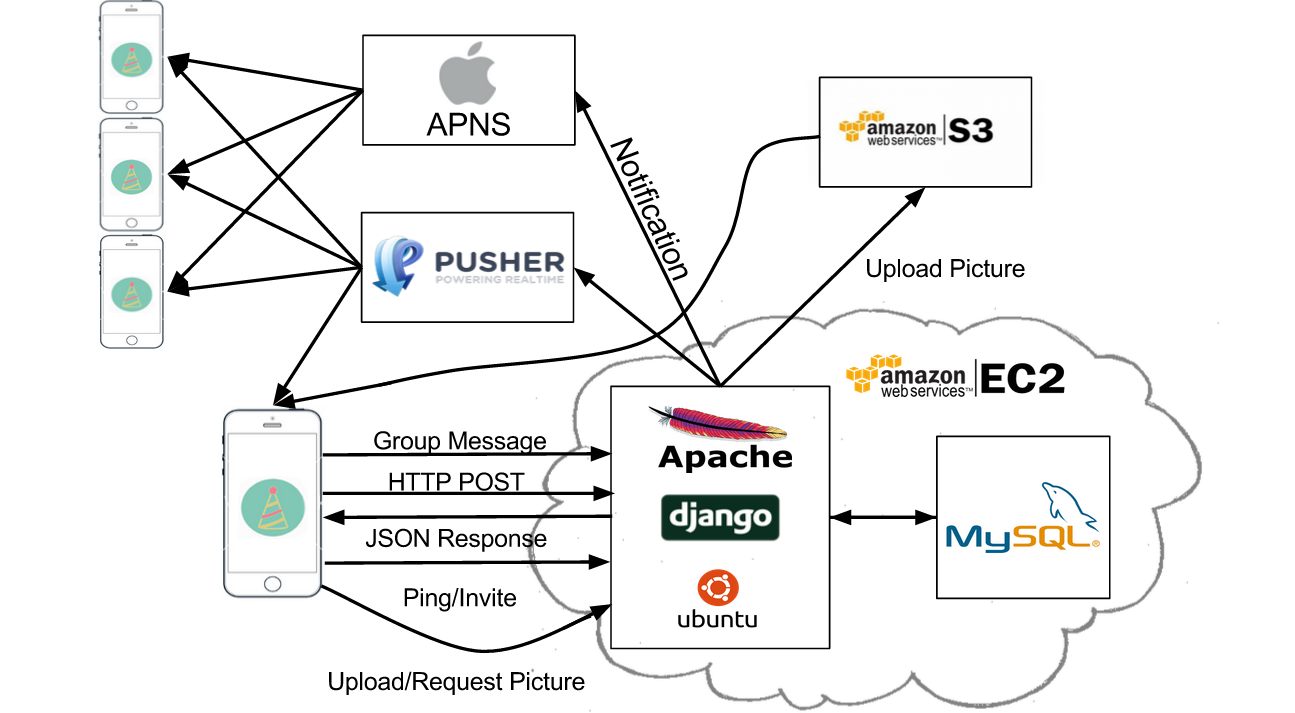
\includegraphics[scale=0.4]{Stack.png}
    \caption{
        A simplified map of the PartyUp back end. 
    }
    \label{fig:stack}
\end{figure}


In this section, we will give an overview each of major components in this system
in the context of the code found in the
backend-333 directory (\url{https://github.com/BDGL-Hacks/backend-333}).
At the top level, there are a few files and sub-directories.

\texttt{curl.sh} is a short bash script that is basically a wrapper for 
\texttt{cURL} that makes it a little easier to test the back end API.

\texttt{requirements.txt} is a list of Python packages that are needed to
run all of the Python programs within the directory.

The two directories, \texttt{testdata} and \texttt{partyup} will be covered
in greater detail below.
It should noted that all of the Python files included in these directories
are written according to the PEP-8 Python standard.

\subsection{PartyUp's requirements}

The biggest third-party packages that we used for PartyUp are a package for Pusher, a package for Push Notifications, and MySQL-python. 
The file \texttt{requirements.txt} includes the names and versions of each package used.
All of the packages can be installed using \texttt{pip}, the recommended
Python package manager.
The command
\begin{lstlisting}
    pip install -r requirements.txt
\end{lstlisting}
will install all of the packages at once.

\subsection{testdata}

This directory contains a Python script, \texttt{filldatabase.py},
which can be used to fill the PartyUp database with test data
found in the accompanying files, \texttt{users.txt} and \texttt{events.txt}.
The files themselves are well documented and contain information about
how to run the script.

\subsection{partyup}

This directory contains the Django project, and thus,
it contains most of the code for the back end.
For the most part, the files are structured in the way you would
expect in your typical Django project
(see \url{https://docs.djangoproject.com/en/1.7/} for an introduction to Django),
although there are a few exceptions.

\subsubsection{The \texttt{users} app}

All of the backend API code is contained within the \texttt{users} app.
The \texttt{models.py} file contains all of the Django objects and their relations for our database. 
The views (HTTP responses) for all of our API calls are found in the \texttt{views} folder and are split into appropriate files.
The code is split into the files in the same manner that the API calls are divided within our GitHub wiki. 
We believed the best way to keep relevant API calls together was to group them by the objects that they interacted with. 
More information on individual methods can be found on our wiki or in the code comments.

\subsubsection{Our Django Models}

Our main models are \texttt{User\_Profile}, \texttt{Group}, and \texttt{Event}. 
We also have a few helper models. 
Our \texttt{Channel} model stores the information for each \texttt{Group}'s chat channel. 
The Pusher channel that a \texttt{Channel} posts on is defined by the string \texttt{GroupChat} and the group's ID. (e.g. \texttt{GroupChat112}) 
Our \texttt{Message} model is a single message sent in the chat. 
Our \texttt{Ping} model is the information corresponding with a single safety ping. 
Finally, our \texttt{User\_Group\_info} model contains information about the relationship of a \texttt{User} and \texttt{Group} (e.g. which \texttt{Event} the \texttt{User} is at for a single \texttt{Group}).

We have one third-party model which is \texttt{APNSDevice}, or Apple Push Notification Services Device. 
These models are created when a user logs in and they are used to send push notifications to an iOS device.

\subsubsection{Third Party API keys}

Because API keys are sensitive information, none of them are included in the git repositories. 
If you would like to receive the API keys, either get them from the server or ask a current group member.

\section{Implementation: Django HTML views}

Because of time constraints, some of the app's views are rendered in HTML. We created these views in the back end repository and they can be found in the Django app \texttt{web} in the \texttt{partyup} directory. The css and js files that we created are found in the  \texttt{static} directory and the HTML files are found in the  \texttt{templates} directory. The frameworks that we used are Bootstrap's carousel, Bootstrap's glyphicons, Google's fonts, jQuery, and jQuery mobile. 

\end{document}
